\documentclass[12pt]{article}
%\usepackage[utf8]{inputenc}
%\documentclass[UTF8]{ctexart}
%\usepackage[UTF8, heading = false, scheme = plain]{ctex}
\usepackage{geometry}
%geometry{a4paper,scale=0.9}
\geometry{a4paper,left=1cm,right=1cm,top=1cm,bottom=2cm}
\usepackage{amsfonts}
\usepackage{color}
\usepackage{url}
%\usepackage{biblatex}
\usepackage{amsmath}
\usepackage{amssymb}
\usepackage{latexsym}
\usepackage{cite}
%\addbibresource{ref.bib}
%\bibliography{ref.bib}
\usepackage{caption}
\usepackage{graphicx, subfig}
\usepackage{float}
%\usepackage[fontset=ubuntu]{ctex}
%\usepackage{fontspec}
\usepackage{xeCJK}
%\usepackage[colorlinks,
%anchorcolor=black,
%citecolor=black]{hyperref}
%\setmainfont{SimSun}
\usepackage[section]{placeins}
\usepackage{enumitem}
\usepackage{framed}
\usepackage[framemethod=TikZ]{mdframed}
\usepackage{indentfirst}
\usepackage{setspace}%使用间距宏包
\linespread{1.5}
%\title{预备知识}
%\author{leolinuxer }
%\date{June 2020}

\title{从极大似然到EM\cite{ML_EM_Algorithm_Detailed}\cite{EM_Algorithm_Tutorial}\cite{Everyone_Knows_EM_Algorithm}}
\author{leolinuxer}
%\date{June 2020}

\begin{document}
%\setlength{\parindent}{0pt}
\maketitle
\tableofcontents

\section{极大似然}
\subsection{问题描述}
假设我们需要调查我们学校学生的身高分布。我们先假设学校所有学生的身高服从正态分布$N(\mu, \sigma^2)$ 。(注意:\textbf{极大似然估计的前提一定是要假设数据总体的分布,如果不知道数据分布,是无法使用极大似然估计的}),这个分布的均值 $\mu$ 和方差$\sigma^2$ 未知,如果我们估计出这两个参数,那我们就得到了最终的结果。那么怎样估计这两个参数呢?

学校的学生这么多,我们不可能挨个统计吧?这时候我们需要用到概率统计的思想,也就是抽样,根据样本估算总体。假设我们随机抽到了 200 个人(也就是 200 个身高的样本数据,为了方便表示,下面“人”的意思就是对应的身高)。然后统计抽样这 200 个人的身高。根据这 200 个人的身高估计均值$\mu$ 和方差 $\sigma^2$ 。

用数学的语言来说就是:为了统计学校学生的身高分布,我们独立地按照概率密度 $p(x|\theta)$ 抽取了 200 个(身高),组成样本集 $X = x_1, x_2, \cdots, x_N$ (其中 $x_i$ 表示抽到的第 $i$ 个人的身高,这里 N 就是 200,表示样本个数),我们想通过样本集 $X$ 来估计出总体的未知参数$\theta$ 。这里概率密度 $p(x|\theta)$ 服从高斯分布$N(\mu, \sigma^2)$,其中的未知参数是$\theta=[\mu, \sigma]^T$ 。

那么问题来了怎样估算参数$\theta$呢?

\subsection{估算参数}
我们先回答几个小问题:

\textbf{问题一:抽到这 200 个人的概率是多少呢?}

由于每个样本都是独立地从 $p(x|\theta)$ 中抽取的,换句话说这 200 个学生随便捉的,他们之间是没有关系的,即他们之间是相互独立的。假如抽到学生 A(的身高)的概率是 $p(x_A|\theta)$,抽到学生B的概率是 $p(x_B|\theta)$,那么同时抽到男生 A 和男生 B 的概率是 $p(x_A|\theta) \times p(x_B|\theta)$,同理,我同时抽到这 200 个学生的概率就是他们各自概率的乘积了,即为他们的联合概率,用下式表示:
$$
L(\theta)  = L(x_1, x_2, \cdots, x_n; \theta) = \prod_{i=1}^np(x_i|\theta), \quad \theta \in \Theta
$$

$n$ 为抽取的样本的个数,本例中 $n=200$,这个概率反映了,在概率密度函数的参数是$\theta$时,得到 $X$ 这组样本的概率。上式中等式右侧只有$\theta$是未知数,所以 L 是 $\theta$ 的函数。

这个函数反映的是在不同的参数$\theta$ 取值下,取得当前这个样本集的可能性,因此称为参数 $\theta$ 相对于样本集 $X$ 的似然函数(likelihood function),记为$L(\theta)$ 。

对 $L$ 取对数,将其变成连加的,称为对数似然函数,如下式:
$$
H(\theta) = \ln L(\theta) = \ln \prod_{i=1}^np(x_i|\theta) = \sum_{i=1}^n\ln p(x_i|\theta)
$$

\textbf{问题二:学校那么多学生,为什么就恰好抽到了这 200 个人 ( 身高) 呢?}

在学校那么学生中,我一抽就抽到这 200 个学生(身高),而不是其他人,那是不是表示在整个学校中,这 200 个人(的身高)出现的概率极大啊,也就是其对应的似然函数 $L(\theta)$ 极大,即
$$
\hat{\theta} = \arg\max L(\theta)
$$

$\hat{\theta} $ 这个叫做$\theta$ 的极大似然估计量,即为我们所求的值。

\textbf{问题三:那么怎么极大似然函数?}

求 $L(\theta)$ 对所有参数的偏导数,然后让这些偏导数为 0,假设有$n$个参数,就有 $n$ 个方程组成的方程组,那么方程组的解就是似然函数的极值点了,从而得到对应的 $\theta$ 了。

\subsection{极大似然估计总结}
极大似然估计你可以把它看作是一个反推。多数情况下我们是根据已知条件来推算结果,而极大似然估计是已经知道了结果,然后寻求使该结果出现的可能性极大的条件,以此作为估计值。

比如说,
\begin{itemize}
\setlength{\itemsep}{0pt}
\setlength{\parsep}{0pt}
\setlength{\parskip}{0pt}
    \item 假如一个学校的学生男女比例为 9:1 (条件),那么你可以推出,你在这个学校里更大可能性遇到的是男生 (结果);
    \item 假如你不知道那女比例,你走在路上,碰到100个人,发现男生就有90个 (结果),这时候你可以推断这个学校的男女比例更有可能为 9:1 (条件),这就是极大似然估计。
\end{itemize}

极大似然估计,只是一种概率论在统计学的应用,它是参数估计的方法之一。说的是已知某个随机样本满足某种概率分布,但是其中具体的参数不清楚,通过若干次试验,观察其结果,利用结果推出参数的大概值。

极大似然估计是建立在这样的思想上:已知某个参数能使这个样本出现的概率极大,我们当然不会再去选择其他小概率的样本,所以干脆就把这个参数作为估计的真实值。

\subsection{求极大似然函数估计值的一般步骤}
\begin{itemize}
\setlength{\itemsep}{0pt}
\setlength{\parsep}{0pt}
\setlength{\parskip}{0pt}
    \item 写出似然函数;
    \item 对似然函数取对数,并整理;
    \item 求导数,令导数为 0,得到似然方程;
    \item 解似然方程,得到的参数。
\end{itemize}

\subsection{极大似然函数的应用}
\subsubsection{回归问题中的极小化平方和 (极小化代价函数)}
假设线性回归模型具有如下形式: 
$$
h(x) = \sum_{i=1}^d\theta_jx_j + \epsilon = \theta^Tx + \epsilon
$$

其中 $x \in \mathbf{R}^{1\times d}, \theta \in \mathbf{R}^{1\times d}$,$X = (x_1, \cdots, x_m)^T \in \mathbf{R}^{m\times d}, y \in \mathbf{R}^{m \times 1}$,误差 $\epsilon \in \mathbf{R}$。如何求 $\theta$ 呢?

\begin{itemize}
\setlength{\itemsep}{0pt}
\setlength{\parsep}{0pt}
\setlength{\parskip}{0pt}
    \item 最小二乘估计:最合理的参数估计量应该使得模型能最好地拟合样本数据,也就是估计值和观测值之差的平方和最小,其推导过程如下所示:
    $$
    J(\theta) = \sum_{i=1}^m\Big(h_{\theta}(x_i) - x\Big)^2
    $$
    求解方法是通过梯度下降算法,训练数据不断迭代得到最终的值。

    \item 极大似然法:最合理的参数估计量应该使得从模型中抽取 $m$ 组样本观测值的概率极大,也就是似然函数极大。

假设误差项$\epsilon \in N(\mu, \sigma^2)$ ,则 $y_i \in N(\theta x_i, \sigma^2)$(建议复习一下正态分布的概率密度函数和相关的性质):
\begin{align*}
p(y_i|x_i; \theta) &= \frac{1}{\sqrt{2\pi}\sigma}\exp\Big(-\frac{(y_i - \theta^Tx_i)^2}{2\sigma^2}\Big) \\
L(\theta) &= \prod_{i=1}^mp(y_i|x_i;\theta) \\
	&= \prod_{i=1}^m\frac{1}{\sqrt{2\pi}\sigma}\exp\Big(-\frac{(y_i - \theta^Tx_i)^2}{2\sigma^2}\Big) \\
H(\theta) &= \log(L(\theta)) \\
	&= \log\prod_{i=1}^m\frac{1}{\sqrt{2\pi}\sigma}\exp\Big(-\frac{(y_i - \theta^Tx_i)^2}{2\sigma^2}\Big) \\
	&= \sum_{i=1}^m\Bigg(\log\bigg(\frac{1}{\sqrt{2\pi}\sigma}\exp\Big(-\frac{(y_i - \theta^Tx_i)^2}{2\sigma^2}\Big)\bigg)\Bigg) \\
	&= -\frac{1}{2\sigma^2}\sum_{i=1}^m(y_i - \theta^Tx_i)^2 - m\ln \sigma\sqrt{2\pi}
\end{align*}

令 $J(\theta) = \frac{1}{2}\sum_{i=1}^m(y_i - \theta^
Tx_i)^2$,则 $\arg\max_\theta \Leftrightarrow \arg\min_\theta J(\theta)$, 即将极大似然函数等价于极小化代价函数。
\end{itemize}

这时可以发现,此时的极大化似然函数和最初的最小二乘损失函数的估计结果是等价的。但是要注意这两者只是恰好有着相同的表达结果,原理和出发点完全不同。

\subsubsection{分类问题中极小化交叉熵 (极小化代价函数)}
在分类问题中,交叉熵的本质就是似然函数的极大化,逻辑回归的假设函数为:
$$
h(x) = \hat{y} = \frac{1}{1 + e^{-\theta^Tx + b}}
$$

根据之前学过的内容我们知道 $\hat{y} = p(y = 1|x, \theta)$:
\begin{itemize}
\setlength{\itemsep}{0pt}
\setlength{\parsep}{0pt}
\setlength{\parskip}{0pt}
    \item 当 $y = 1$ 时,$p_1 = p(y = 1|x, \theta) = \hat{y}$
    \item 当 $y = 0$ 时,$p_1 = p(y = 0|x, \theta) = 1 - \hat{y}$
\end{itemize}

合并上面两式子,可以得到
$$
p(y|x, \theta) = \hat{y}^y(1-\hat{y})^{1-y}
$$
\begin{align*}
L(\theta) &= \prod_{i=1}^mp(y_i|x_i; \theta) \\
	&= \prod_{i=1}^m \hat{y}_i^y(1-\hat{y}_i)^{1-y} \\
H(\theta) &= \log(L(\theta)) \\
	&= \log\prod_{i=1}^m \hat{y}_i^y(1-\hat{y}_i)^{1-y}  \\
	&= \sum_{i=1}^m\log{\hat{y_i}^y(1-\hat{y}_i)^{1-y} } \\
	&= \sum_{i=1}^my_i\log \hat{y}_i + (1- y_i)\log(1-\hat{y}_i)
\end{align*}

令 $J(\theta) = -H(\theta) = -sum_{i=1}^my_i\log \hat{y}_i + (1- y_i)\log(1-\hat{y}_i)$,则 $\arg\max_\theta H(\theta) \Leftrightarrow \arg\min_\theta J(\theta)$, 即将极大似然函数等价于极小化代价函数。

\section{EM 算法的思想}
EM 算法,全称 Expectation Maximization Algorithm。期望最大算法是一种迭代算法,用于\textbf{含有隐变量}(Hidden Variable)的概率参数模型的最大似然估计或极大后验概率估计。

EM 算法的核心思想非常简单,分为两步:Expection-Step 和 Maximization-Step。E-Step 主要通过观察数据和现有模型来估计参数,然后用这个估计的参数值来计算上述对数似然函数的期望值;而 M-Step 是寻找似然函数最大化时对应的参数。由于算法会保证在\textbf{每次迭代之后似然函数都会增加},所以函数最终会收敛。

\section{EM 算法举例}
\subsection{例子 A}
第一个例子我们将引用 Nature Biotech 的 EM tutorial 文章中的例子。

\subsubsection{背景}
假设有两枚硬币 A 和 B,他们的随机抛掷的结果如下图所示:
\begin{figure}[H]
    \centering
    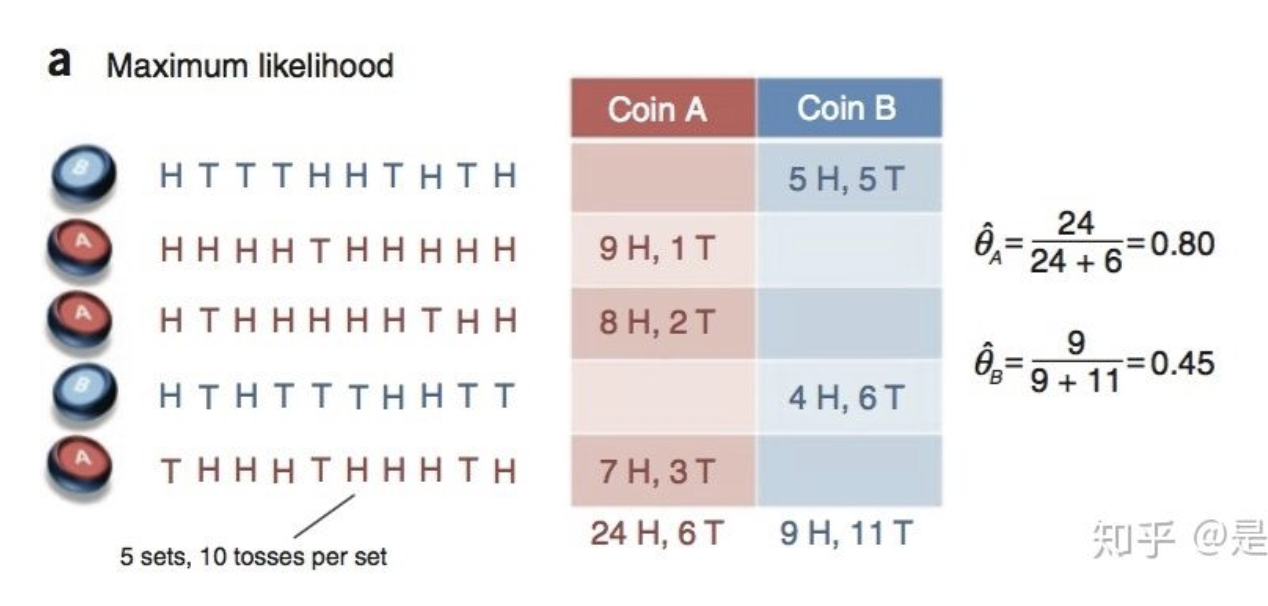
\includegraphics[width=.8\textwidth]{fig/EM_Detailed_Example_A_1.png}
\end{figure}
定义如下符号:
\begin{itemize}
\setlength{\itemsep}{0pt}
\setlength{\parsep}{0pt}
\setlength{\parskip}{0pt}
    \item $\theta$:得到正面的概率;
    \item $\theta_A$:硬币A得到正面的概率;
    \item $\theta_B$:硬币B得到正面的概率;
\end{itemize}

我们很容易估计出两枚硬币抛出正面的概率:
$$
\theta_A = 24/30 = 0.8
$$
$$
\theta_B = 9/20 = 0.45
$$

现在我们加入隐变量,抹去每轮投掷的硬币标记:
\begin{figure}[H]
    \centering
    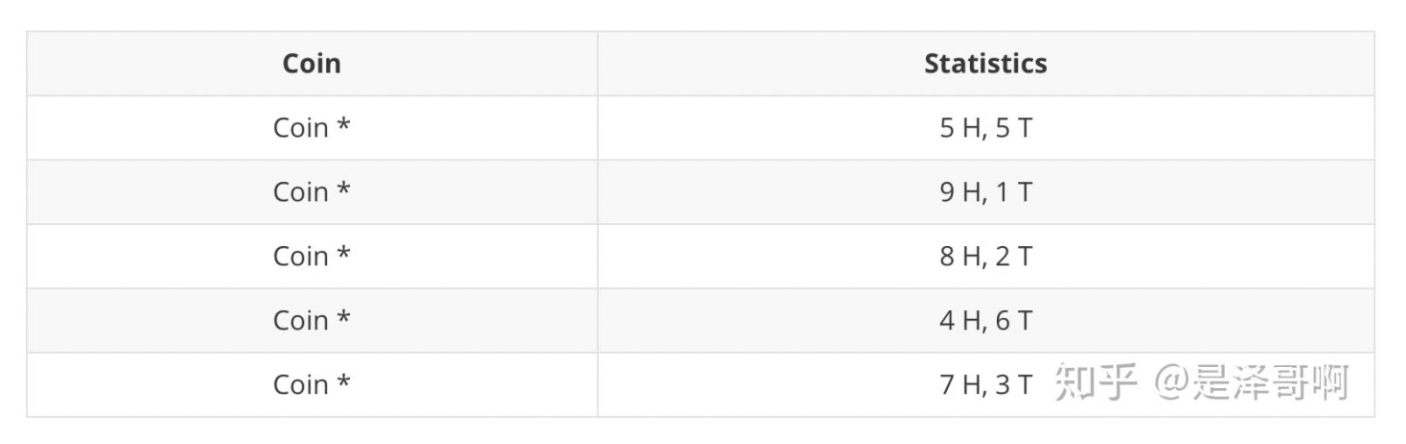
\includegraphics[width=.8\textwidth]{fig/EM_Detailed_Example_A_2.png}
\end{figure}

碰到这种情况,我们该如何估计 $\theta_A$ 和 $\theta_B$ 的值?

我们多了一个隐变量 $Z = (z_1, z_2, z_3, z_4, z_5)$ ,代表每一轮所使用的硬币。我们需要知道每一轮抛掷所使用的硬币$z_i$,这样才能估计 $\theta_A$ 和 $\theta_B$ 的值,但是估计隐变量 $Z$ 我们又需要知道  $\theta_A$  和 $\theta_B$ 的值,才能用极大似然估计法去估计出 $Z$。这就陷入了一个鸡生蛋和蛋生鸡的问题。

其解决方法就是先随机初始化 $\theta_A$  和 $\theta_B$,然后用去估计 $Z$, 然后基于 $Z$ 按照最大似然概率去估计新的 $\theta_A$  和 $\theta_B$,循环至收敛。

\subsubsection{计算}
随机初始化 $\theta_A = 0.6$  和 $\theta_B = 0.5$。


对于第一轮来说,记 5 正 5 反 这一事件为$Y$。

如果是硬币 A,得出事件 $Y$ 的概率为:
$$
P(Y|Z=A) = (\theta_A)^5 * (1-\theta_A)^5 = 0.6^5*0.4^5
$$

如果是硬币 B,得出事件 $Y$ 的概率为: 
$$
P(Y|Z=B) = (\theta_B)^5 * (1-\theta_B)^5 = 0.5^5*0.5^5
$$

根据全概率公式,有:
$$
P(Y) = P(Y|Z=A)P(Z=A) + P(Y|Z=B)P(Z=B) = 0.6^5*0.4^5*0.5 + 0.5^5*0.5^5*0.5
$$

根据贝叶斯定理,可以算出使用的是硬币 A 的概率为:
$$
P(Z=A|Y) = P(Z=A)\frac{P(Y|Z=A)}{P(Y)} = 0.5 * \frac{0.6^5*0.4^5}{0.6^5*0.4^5*0.5 + 0.5^5*0.5^5*0.5} = 0.45
$$

可以算出使用的是硬币 B 的概率为:
$$
P(Z=A|Y) = P(Z=A)\frac{P(Y|Z=A)}{P(Y)} = 0.5 * \frac{0.5^5*0.5^5}{0.6^5*0.4^5*0.5 + 0.5^5*0.5^5*0.5} = 0.55$$

从期望的角度来看,对于第一轮抛掷,使用硬币 A 的概率是 0.45,使用硬币 B 的概率是 0.55。其他轮同理。\textbf{这一步我们实际上是估计出了 Z 的概率分布,这步就是 E-Step}。
\begin{figure}[H]
    \centering
    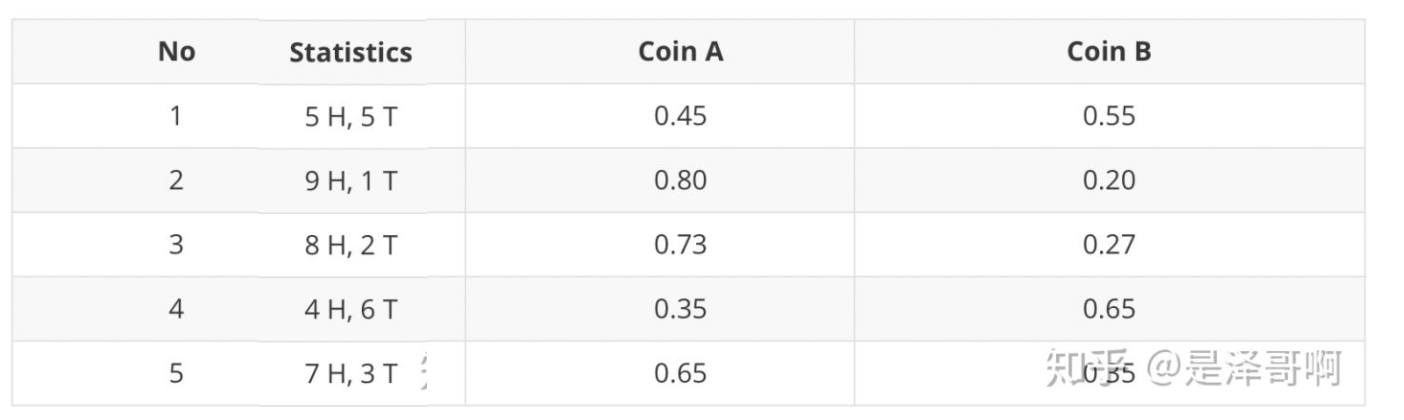
\includegraphics[width=.8\textwidth]{fig/EM_Detailed_Example_A_3.png}
\end{figure}

结合硬币 A 的概率和上一轮投掷结果,我们利用期望可以求出硬币 A 和硬币 B 的贡献。以第二轮硬币 A 为例子,计算方式为:
$$
H: 0.80 * 9 = 7.2; \ T = 0.80 * 1 = 0.80
$$

于是我们可以得到:
\begin{figure}[H]
    \centering
    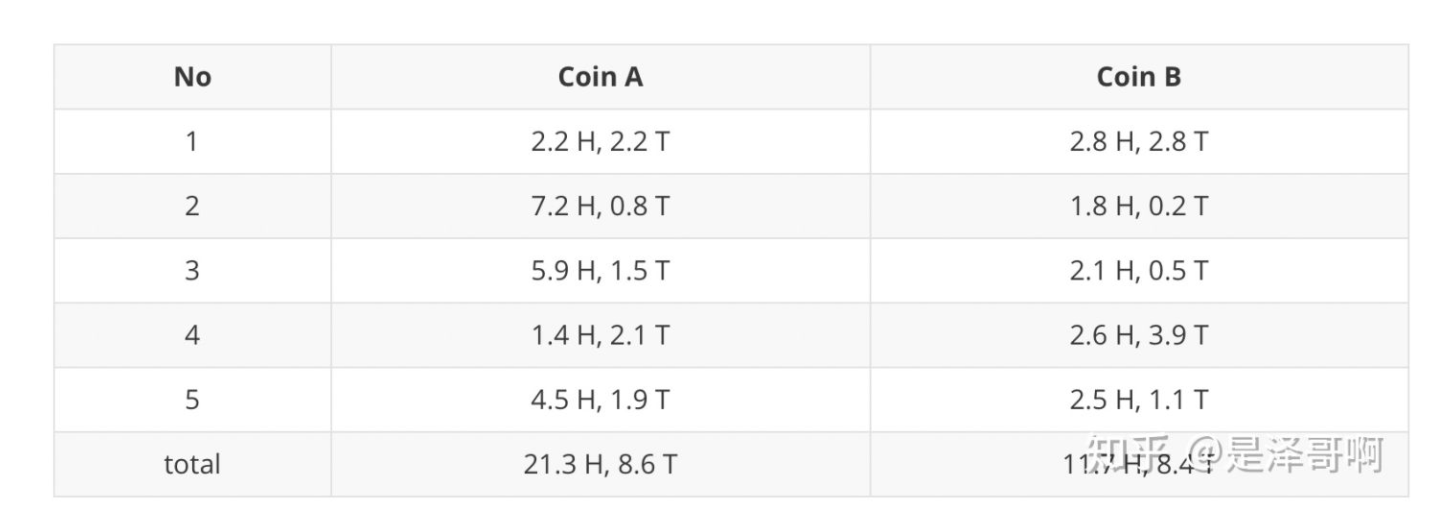
\includegraphics[width=.8\textwidth]{fig/EM_Detailed_Example_A_4.png}
\end{figure}


然后用极大似然估计来估计新的 $\theta_A$  和 $\theta_B$。
$$
\theta_A = \frac{21.3}{21.3+8.6} = 0.71
$$
$$
\theta_A = \frac{11.7}{11.7+8.4} = 0.58
$$

\textbf{这步就对应了 M-Step,重新估计出了期望值}。如此反复迭代,我们就可以算出最终的参数值。

\subsection{例子 B}
现在一个班里有 50 个男生和 50 个女生,且男女生分开。我们假定男生的身高服从正态分布: $N(\mu_1, \sigma_1^2)$,女生的身高则服从另一个正态分布: $N(\mu_2, \sigma_2^2)$ 。这时候我们可以用极大似然法(MLE),分别通过这 50 个男生和 50 个女生的样本来估计这两个正态分布的参数。

但现在我们让情况复杂一点,就是这 50 个男生和 50 个女生混在一起了。我们拥有 100 个人的身高数据,却不知道这 100 个人每一个是男生还是女生。

这时候情况就有点尴尬,因为通常来说,我们只有知道了精确的男女身高的正态分布参数我们才能知道每一个人更有可能是男生还是女生。但从另一方面去考量,我们只有知道了每个人是男生还是女生才能尽可能准确地估计男女各自身高的正态分布的参数。

这个时候有人就想到我们必须从某一点开始,并用迭代的办法去解决这个问题:我们先设定男生身高和女生身高分布的几个参数(初始值),然后根据这些参数去判断每一个样本(人)是男生还是女生,之后根据标注后的样本再反过来重新估计参数。之后再多次重复这个过程,直至稳定。这个算法也就是 EM 算法。

\section{EM 算法推导}
\subsection{推导过程}
给定数据集,假设样本间相互独立,我们想要拟合模型 $p(x;\theta)$ 到数据的参数。根据分布我们可以得到如下似然函数:
$$
L(\theta) = \sum_{i=1}^n\log{p(x_i;\theta)} = \sum_{i=1}^n\log\Big(\sum_zp(x_i, z;\theta)\Big)
$$

第一步是对极大似然函数取对数,第二步是对每个样本的每个可能的类别 z 求联合概率分布之和。\textbf{如果这个 z 是已知的数,那么使用极大似然法会很容易。但如果 z 是隐变量,我们就需要用 EM 算法来求}。

事实上,隐变量估计问题也可以通过梯度下降等优化算法,但事实由于求和项将随着隐变量的数目以指数级上升,会给梯度计算带来麻烦;而 EM 算法则可看作一种非梯度优化方法。

对于每个样本 $i$,我们用 $Q_i(z)$ 表示样本 $i$ 隐含变量 $z$ 的某种分布,且 $Q_i(z)$ 满足条件 $\sum_z^ZQ_i(z) = 1, Q_i(z) \ge 0$。

我们将上面的式子做以下变化:
\begin{align*}
L(\theta) = \sum_i^n\log{p(x_i; \theta)} &=  \sum_i^n\log\Big(\sum_z^Zp(x_i, z;\theta)\Big) \\
	&= \sum_i^n\log\Big(\sum_z^ZQ_i(z)\frac{p(x_i, z;\theta)}{Q_i(z)}\Big) \\
	&\ge \sum_i^n\sum_z^ZQ_i(z)\log\frac{p(x_i, z;\theta)}{Q_i(z)} \qquad (\text{Jensen 不等式})
\end{align*}

上面式子中,第一步是求和每个样本的所有可能的类别 z 的联合概率密度函数,但是这一步直接求导非常困难,所以将其分母都乘以函数 $Q_i(z)$ ,转换到第二步。从第二步到第三步是利用 Jensen 不等式。解释如下:

因为对数函数是凹函数,所以有:
$$
\log\Big(\sum_z^Z{Q_i(z)\frac{p(x_i,z;\theta)}{Q_i(z)}}\Big) \ge \sum_z^ZQ_i(z)\log{\frac{p(x_i,z;\theta)}{Q_i(z)}}
$$

通过上面我们得到了:$L(\theta) \ge J(z,Q)$ 的形式($z$ 为隐变量),\textbf{那么我们就可以通过不断最大化 $J(z,Q)$ 的下界来使得 $L(\theta)$ 不断提高:}
\begin{itemize}
\setlength{\itemsep}{0pt}
\setlength{\parsep}{0pt}
\setlength{\parskip}{0pt}
    \item 固定$\theta$,调整 $Q(z)$ 使得下界$J(z,Q)$ 不断上升至与 $L(\theta)$ 在点 $\theta$ 处相等;
    \item 然后固定 $Q(z)$,调整 $\theta$ 使得下界$J(z,Q)$ 达到最大值,此时为新的 $\theta$。
    \item 重复上述步骤,直到收敛到似然函数$L(\theta)$ 的最大值处的 $\theta^*$
\end{itemize}

也就是说,EM 算法通过引入隐含变量,使用 MLE(极大似然估计)进行迭代求解参数。通常引入隐含变量后会有两个参数,EM 算法首先会固定其中的第一个参数,然后使用 MLE 计算第二个变量值;接着通过固定第二个变量,再使用 MLE 估测第一个变量值,依次迭代,直至收敛到局部最优解。

\subsection{什么时候下界$J(z,Q)$ 与 $L(\theta)$  相等}
当 $X = E[X]$ 时,即为常数时等式成立,即:
$$
\frac{p(x_i, z;\theta)}{Q_i(z)} = c
$$

做个变换:
$$
\sum_z{p(x_i, z;\theta)} = c\sum_z{Q_i(z)}
$$

其中 $\sum{Q_i(z)} = 1$ ,所以可以推导出:
$$
\sum_z{p(x_i, z;\theta)} = c
$$

因此得到了:
\begin{align*}
Q_i(z) &= \frac{p(x_i, z;\theta)}{\sum_zp(x_i, z;\theta)} \\
	&= \frac{p(x_i, z;\theta)}{p(x_i;\theta)} \\
	&= p(z|x_i;\theta)
\end{align*}

至此我们推出了在固定参数下,使下界拉升的 $Q(z)$ 的计算公式,也就是后验概率,同时解决了 $Q(z)$ 如何选择的问题。这就是我们刚刚说的 EM 算法中的 E-Step,目的是建立$L(\theta)$的下界。接下来得到 M-Step 目的是在给定 $Q(z)$ 后调整$\theta$ ,从而极大化似然函数 $L(\theta)$ 的下界$J(z,Q)$ 。

\subsection{为什么一定会收敛?}
这边简单说一下,因为每次 $\theta$ 更新时(每次迭代时),都可以得到更大的似然函数,也就是说极大似然函数时单调递增,那么我们最终就会得到极大似然估计的最大值。

但是要注意,迭代一定会收敛,但不一定会收敛到真实的参数值,因为可能会陷入局部最优。所以 EM 算法的结果很受初始值的影响。

%\printbibliography
\bibliography{../ref}
\bibliographystyle{IEEEtran}
\end{document}
